\documentclass[12pt,answers]{exam}

\usepackage{amsmath,amsfonts,amssymb,mathtools,physics,commath}
\usepackage{float}
\usepackage{todonotes}
\newcommand{\vect}[1]{\left\langle #1\right\rangle}
\newcommand{\inv}{^{-1}}

\newcommand{\vbd}{\vb{d}}
\newcommand{\vbi}{\vb{i}}
\newcommand{\vbj}{\vb{j}}
\newcommand{\vbk}{\vb{k}}
\newcommand{\vbn}{\vb{n}}
\newcommand{\vbr}{\vb{r}}
\newcommand{\vbu}{\vb{u}}
\newcommand{\vbv}{\vb{v}}
\newcommand{\vbw}{\vb{w}}

\DeclareMathOperator{\proj}{proj}

\pagestyle{headandfoot}
\firstpageheadrule
\runningheadrule
\firstpageheader{Math 222}{Exam 1|Solutions, Page \thepage\ of \numpages}{2021 Fall}
\runningheader{Math 222}{Exam 1|Solutions, Page \thepage\ of \numpages}{2021 Fall}
\runningfooter{}{}{}

% \title{2021 Fall Calc 3 Final Exam|Solutions}
% \author{Winston Cheong}
% \date{}

\begin{document}
% \maketitle
\begin{questions}

\question
For the following questions, suppose $\vbu = \vect{1,-1,0}$ and $\vbv = \vect{0,-1,1}$.
\begin{parts}

  \part[5] Evaluate $\vbu - 3\vbv$.
  \begin{solution}
    $=\vect{1,-1,0}-3\vect{0,-1,1} = \boxed{\vect{1,2,-3}}$
  \end{solution}

  \part[5] Evaluate $\vbu \vdot \vbv$.
  \begin{solution}
    $=1(0)+(-1)(-1)+0(1) = \boxed{1}$
  \end{solution}

  \part[5] Find the angle between $\vbu$ and $\vbv$.
  \begin{solution}
    \begin{align*}
      \cos \theta &= \frac{\vbu\vdot\vbv}{\norm{\vbu}\,\norm{\vbv}} = \frac{1}{\sqrt{2} \sqrt{2}} = \frac12 \\ 
      \implies \theta &= \cos\inv \frac12 = \boxed{\frac\pi3}
    \end{align*}
  \end{solution}

  \part[5] Evaluate $\vbu\cross\vbv$.
  \begin{solution}
    $\vbu \cross \vbv = \mqty| \vbi & \vbj & \vbk \\ 1 & -1 & 0 \\ 0 & -1 & 1 | = \boxed{\vect{-1, -1, -1}}$
  \end{solution}

  \part[5] Find the volume of the parallelopiped spanned by $\vbu$, $\vbv$ and the vector $\vect{3,1,-2}$.
  \begin{solution}
    \[
    = \abs{(\vbu\cross\vbv)\vdot\vect{3,1,-2}} 
    = \abs{\vect{-1,-1,-1}\vdot\vect{3,1,-2}} 
    = |-3-1+2| = \boxed{2}
    \]
  \end{solution}

  \newpage
  \part[5] Find the distance between the point $Q = (1,0,0)$ and the line with direction vector $\vbv$ which passes through the point $P = (0,1,0)$.
  \begin{solution}
    The formula for distance can be derived by considering the area of the parallelogram spanned by $\vbv$ and $\overrightarrow{PQ}$:
    \[
      A = \norm{\vbv \cross \overrightarrow{PQ}} = \norm{\vbv} d
      \implies d = \frac{\norm{\vbv \cross \overrightarrow{PQ}}}{\norm{\vbv}}
    \]
    Computing,
    \begin{align*}
      \overrightarrow{PQ} &= \vect{1,-1,0} = \vbu \\ 
      \norm{\vbv \cross \overrightarrow{PQ}} &= \norm{\vbv \cross \vbu} = \norm{\vect{1,1,1}} = \sqrt{3} \\ 
      \norm{\vbv} &= \sqrt 2
    \end{align*}
    so $d = \boxed{\sqrt{\frac32}}$
  \end{solution}
\end{parts}

\newpage
\question
Solve the problems regarding the points $P=(-2,0,1)$, $Q = (0,1,1)$ and $R = (-1,1,0)$.
\begin{parts}
\part[10]
Find a normal vector to the plane containing $P$, $Q$, and $R$.
\begin{solution}
  \begin{align*}
    \overrightarrow{PQ}                            & = \vect{2,1,0}                \\
    \overrightarrow{PR}                            & = \vect{1,1,-1}               \\
    \overrightarrow{PQ} \cross \overrightarrow{PR} & = \mqty| \vbi   & \vbj & \vbk \\ 2 & 1 & 0 \\ 1 & 1 & -1 |  = \boxed{\vect{-1,2,1}} =: \vbn
  \end{align*}
\end{solution}

\part[10]
Write an equation for the plane containing $P$, $Q$ and $R$.
\begin{solution}
  Using the point $P$,
  \begin{align*}
    \vect{-1,2,1}\vdot \vect{x+2,y,z-1} = 0 \\
    -(x+2) + 2y + z-1 = 0                   \\
    -x+2y+z-3 = 0
  \end{align*}
  Any of these works.
\end{solution}

\part[10]
Write an equation for a line passing through $Q$ and perpendicular to the plane found in part (b).
\begin{solution}
  Such a line's direction vector is a scalar of $\vbn$, so a possible equation is
  \[
    \vbr(t) = \vect{0,1,1} + t \vect{-1,2,1}
  \]
\end{solution}

\part[10]
Suppose $S$ is any point on the line found in part (c).
Find the vector projection of $\overrightarrow{PS}$ onto $\overrightarrow{PQ}$.
Explain your response.
\begin{solution}
  Since $S$ is on the line perpendicular to the plane and passing through $Q$, it is effectively ``above'' $Q$. Projecting the point $S$ onto the plane will send it to the point 
  $Q$. 
  Thus, the projection of $\overrightarrow{PS}$ onto $\overrightarrow{PQ}$ is \fbox{$\overrightarrow{PQ}$} itself.
\end{solution}

\end{parts}

\newpage
\question
Sketch and describe the indicated traces of the quadric surface
\[x^2+y+z^2=11\]
\begin{parts}
  \part[5] The $x=1$ trace.
  \begin{solution}
    Setting $x=1$ gives the trace: $y = - z^2 + 10$ which is a parabola:
    \begin{figure}[H]
      \centering
      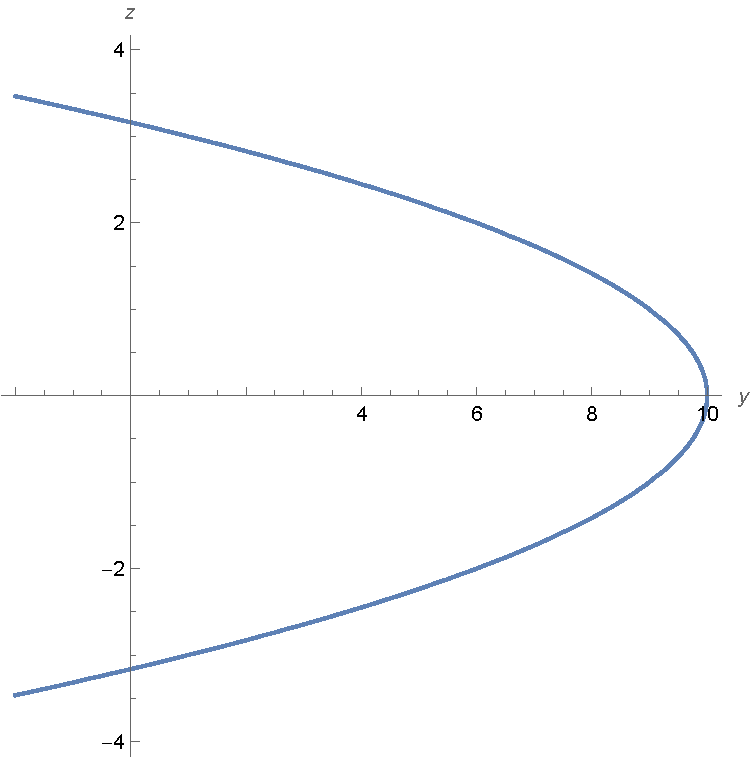
\includegraphics[width=.5\linewidth]{graphics/2021-fall-exam1-3a.pdf}
    \end{figure}
  \end{solution}

  \part[5] The $y=2$ trace.
  \begin{solution}
    Setting $y=2$ gives the trace: $x^2+z^2=9$, which is a circle of radius 3.
    \begin{figure}[H]
      \centering
      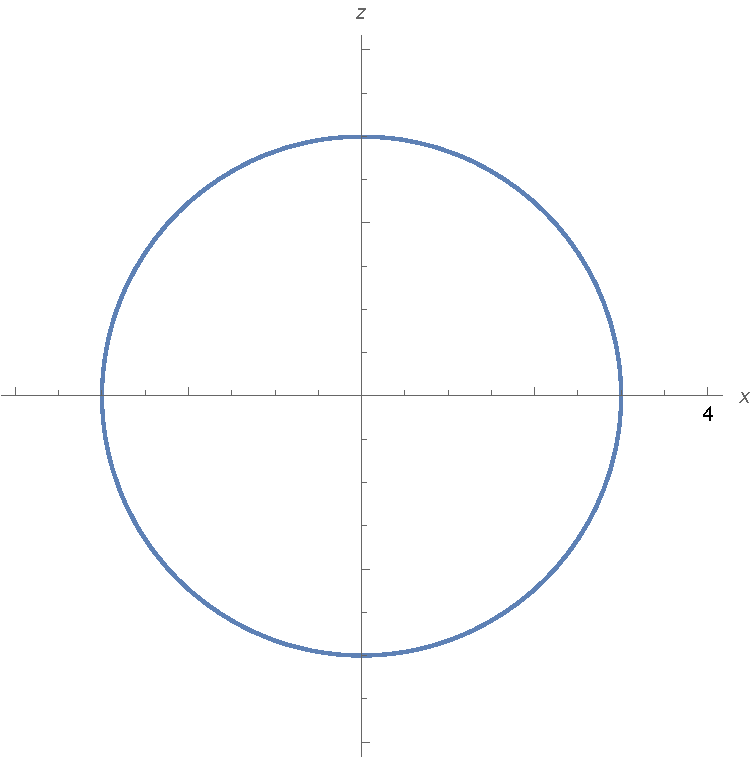
\includegraphics[width=.5\linewidth]{graphics/2021-fall-exam1-3b.pdf}
    \end{figure}
  \end{solution}
  
\end{parts}

\newpage
\question[10] Give the inequalities in Cartesian coordinates that describe the region below given in spherical coordinates
\[
  \rho \le 3, \qquad \frac\pi2 \le \varphi \le \pi, \qquad 0 \le \theta \le \pi
\]
\begin{solution}
  \[
    x^2 + y^2 + z^2 \le 9, \qquad -3 \le z \le 0, \qquad y\ge0
  \]
\end{solution}

\question[10] If it exists, find
\[\lim_{t\to0} \vbr(t)\]
for the vector valued function
\[\vbr(t) = \vect{\frac{e^t-1}{t}, \frac{t+1}{t^2+1}, \ln(t^2+1)} \]
\begin{solution}
  Evaluating the limits for the second and third component functions is straightforward. 
  Evaluating limit for the first component function requires L'H\^{o}pital:
  \[
    \lim_{t\to0} \frac{e^t-1}{t} \overset{L'H}{=} \lim_{t\to0}\frac{e^t}{1} = 1
  \]
  Thus the answer is
  \[
    \boxed{\vect{1,1,0}}
  \]
\end{solution}

\end{questions}
\end{document}
